\documentclass[10pt]{article}

%Packages prioritaires
\usepackage[utf8]{inputenc}  
\usepackage[T1]{fontenc}
\usepackage[francais]{babel}
\usepackage{titlesec}
\usepackage{fancyhdr} % Pour mettre des en-têtes et des pieds de page
\usepackage{array}
\usepackage{graphicx}
\usepackage[margin=0.8in]{geometry}
\usepackage{hyperref}
\usepackage{todonotes}
\title{\Huge{Outil de modélisation de performances des migrations de données inter-cloud}}
\author{\textbf{Antoine Martin - Carole Bonfré} }
\date{Février 2015}

%Param\'{e}trage des pages
\pagestyle{fancy}
\fancyhead[R]{A.Martin \& C.Bonfré}
\fancyhead[L]{MIF20 - TER}
\renewcommand{\headrulewidth}{0.4pt}
\renewcommand{\footrulewidth}{0.4pt}

\renewcommand{\thesection}{\Roman{section}}
\renewcommand{\thesubsection}{\Alph{subsection}}
\renewcommand{\thesubsubsection}{\arabic{subsubsection}}
\titleformat{\subsection}{\bfseries\large}{\hspace{1ex}}{1em}{\thesubsection{} \ }
\titleformat{\subsubsection}{\bfseries\normalsize}{\hspace{2ex}}{1em}{\thesubsubsection{} \ }
\usepackage{xspace}
\newcommand{\KYD}{\textsc{Kyd}\xspace}

\begin{document}

\maketitle

\textbf{Résumé : } Ce projet a pour but de permettre de choisir, selon
une localisation géographique et des paramètres donnés, la meilleure
solution d'hébergement "Cloud" existante. De nombreux chercheurs
rencontrent le besoin de déplacer des Téraoctets de données, cet outil
leur permettra donc d'optimiser la migration de leurs données. À
terme, ce projet Open Source proposera une solution unique sur le
marché.

\section{Introduction}

Dans un monde toujours plus interconnecté, nos données sont de plus en
plus dématérialisées et éparpillées. Nous sommes amenés à les
transférer d’un hébergeur à un autre et dans le but d’optimiser ces
opérations, il nous a été demandé de nous poser différentes questions
concernant l’évaluation des méthodes de transfert.

Cela\todo{YC : Cela quoi ? La thématique, le travail, le stage ?} s’inscrit dans le cadre de l’équipe de recherche Avalon du LIP de
l’ENS de Lyon, qui propose des solutions pour la distribution des
calculs dans des fédérations de Cloud. La distribution de ces calculs
implique de nombreux mouvements de données inter-cloud. Pour
contribuer à l’amélioration des travaux de recherche des membres de
l’équipe Avalon, nous\todo{YC : étudier, proposer, et développer... } allons\todo{YC : pourquoi futur ? C'est maintenant du passé. Donc soit nous avons été amenés à... soit dans ce travail, nous étudions+proposons un outil qui} développer un outil permettant d’évaluer
la performance de transferts de données entre plusieurs hébergeurs de
"Cloud". Cet outil permettra soit d’effectuer des tests de
performances « à la demande », soit de récupérer les résultats déjà
obtenus lors de précédents tests.

Ce projet, nous l’espérons, pourra non seulement aider les chercheurs
de l’équipe Avalon de l’ENS mais également offrir un outil à tous
projets ou personnes ayant besoin d’évaluer les temps de transfert
entre solutions « Cloud » (académiques comme privées).

\section{Recherche et Analyse}
Une première étude des solutions existantes nous aura permis de
sélectionner les outils les plus cohérents pour définir la structure
des données de notre application\todo{YC : Ça fait fumeux et n'apporte pas d'information sur la suite. Si pas utile, on sucre. Sinon mettez de l'information sur ce qui arrive ensuite}.
\subsection{Étude de l'existant}

Cette étude peut être divisée en deux parties. Tout d’abords, nous
avons détaillé les offres de solution de stockage “Cloud” disponibles
sur le marché afin de pouvoir en sélectionner\todo{YC : afin de pouvoir en sélectionner n'apporte pas d'info. Afin d'en dresser les caractéristiques en terme de condition d'achat, performance ou ergonomie ou.. sur le marché}. Nous avons ensuite
cherché un outil déjà capable de réaliser des tests de performances
sur des “Clouds”\todo{YC : jusqu'à présent cloud toujours au singuler (dans inter-cloud par exemple). S'y tenir ou corriger partout} pour justifier\todo{YC : c'est le fait de ne pas l'avoir trouvé qui justifie. Orientez plus haut niveau que votre travail se résumé à du dev de code} le développement de notre propre
outil.

\subsubsection{Solutions de stockage "Clouds"}
\begin{table}[!h]
\caption{Tableau comparatif des "providers"}
\renewcommand{\arraystretch}{1.5}
\begin{center}
\begin{tabular}{|m{1in}|c|m{1in}|m{1in}|m{1in}|m{1in}|c|}
 \hline
 \bf\centering drive & \bf API & \bf Emplacement & \bf Libre & \bf\centering Espace de stockage & \bf Limitation & \bf SDK\\
 \hline
 \centering Dropbox & Oui & S3 & Gratuit / Propriétaire & 2Go & Oui(N/A) & Oui \\
 \hline
  \centering Google drive & Oui  & \href{http://www.google.com/about/datacenters/inside/locations/index.html}{lien} & Gratuit / Propriétaire & 15Go & 10 000 requêtes /jour, 10 requêtes /sec/user & Oui \\
 \hline
  \centering S3 & Oui  &  \href{http://aws.amazon.com/fr/about-aws/global-infrastructure/}{lien} & Gratuit / Propriétaire & 5Go & 20 000 GET, 2 000 PUT / mois & Oui \\
 \hline
  \centering Onedrive & Oui  & ? & Gratuit / Propriétaire & 15Go & Oui (NA) & Oui \\
 \hline
  \centering Cloud Orange & Oui  & Paris (Sénégal ?) & Gratuit / Propriétaire & 10Go à 100Go & Oui (2Go par fichier) & Oui \\
 \hline
  \centering Hubic & Oui  & France (Paris, Roubaix) & Gratuit / Propriétaire & 25Go & Oui (10Go par fichier) & Oui \\
 \hline
  \centering Microsoft Azure & Oui  &  \href{http://azure.microsoft.com/en-us/regions/}{lien} & Gratuit / Propriétaire & 100To & Oui (NA) & Oui \\
 \hline
  \centering iCloud & Oui  & USA (Caroline du Nord) & Gratuit / Propriétaire & 5Go & Oui (15Go par fichier) & Oui \\
 \hline
  \centering Google Cloud Storage & Oui  &  \href{http://www.google.com/about/datacenters/inside/locations/index.html}{lien}  & Payant  / Propriétaire & 1To & Oui 5Tb par fichier & Oui \\
 \hline
  \centering Cloud bouygues & Non  & USA (Pogoplug) & Payant  / Propriétaire & 5Gb & Oui (NA) & Non \\
 \hline
  \centering SFR cloud & Non & Paris & Payant / Propriétaire & 100Go & Oui (NA) & Non \\
 \hline
\end{tabular}
\end{center}
\end{table}

*La mention Oui(N/A) pour la colonne des limitations signifie une
présence de limitation non explicitée par l'hébergeur.

Nous avons remarqué lors de notre analyse que l’hébergeur Dropbox
utilise en fait les services d'Amazon S3. Dropbox étant un des
services les plus populaires, nous avons décidé de le choisir tout de\todo{YC : perso, tout de même -- et + ':'}
même car il apporte probablement des services supplémentaires. Nous
pensons qu’il est également intéressant de tester les différences de
performance entre Amazon S3 et Dropbox. Pour les mêmes raisons, il aurait
également été intéressant de pouvoir vérifier les différences entre
Google Drive et Google Cloud Storage.

Nous avons aussi étudié la possibilité de sélectionner OwnCloud parmi
les hébergeurs (mais l’utilisateur doit posséder une machine avec
OwnCloud installé\todo{YC : comme il doit avoir un compte drive. Présentez Owncloud comme une solution libre pour mettre en place un cloud privé. Owncloud doit même proposer des comptes Owncloud sur leur site, non?}). Il ne possède pas de limitations particulières,
l’espace de stockage est “infini” (il dépend du serveur)\todo{YC : en fait, chacun a un compte sur Owncloud. Les quotas peuvent être mis en place...}, et nous
avons trouvé un SDK développé par un tiers qui semble exploitable pour
notre application. À terme, l’ajout de OwnCloud peut donc être
envisagé. Après analyse des différents acteurs du marché de stockage
en ligne, nous avons décidé de sélectionner les trois hébergeurs
suivant : Dropbox, Amazon S3 et Google Drive\todo{YC : pourquoi ? En raison de leur popularité ?}. Ils possèdent tous les
trois des SDK qui facilitent le développement de notre outil. En
revanche, les espaces de stockage sont parfois assez limités. Nous
souhaiterions, à terme\todo{YC : attention, mot qui revient bcp}, ajouter Google Cloud Storage pour les raisons
citées précédemment.

\subsubsection{Solutions d'évaluation de performance des stockages "Cloud"}

Trois projets ont été identifiés durant cette étude. Le premier, HP
Performance, est une solution propriétaire payante. Parmi de nombreux
outils, elle propose de se placer dans une zone géographique pour
provisionner un générateur de charges (il est donc possible de
chercher le meilleur emplacement)\todo{YC : pas top clair pour le lecteur lambda}. Le second projet, COSBench, est une
solution libre mais plutôt limitée puisqu’elle ne concerne que Swift
Storage et Amazon S3. Elle permet d'exécuter des tâches sur des outils
distants et de les surveiller\todo{YC : Quel est le rapport avec ce que vous faîtes ? Prise de perf ?}. Enfin, CloudScreener est une solution
payante que nous n’avons pas pu tester (nous ne connaissons donc pas
la précision de cet outil\todo{YC : mais vous pouvez décrire un peu ses fonctionnalités ? Que le lecteur comprenne pourquoi vous le citez ici, en quoi votre outil répond à des trucs qu'eux ne font pê pas}). Nous les avons comparés à notre projet
baptisé \KYD (Know Your Data)\todo{YC : ça serait bien de parler en début que le lecteur peut trouver un résumé des caractéristiques de projets... et d'y faire référence ! (avec les commandes ref et label)}.
\newpage

\begin{table}[h]
\caption{Tableau comparatif des solutions trouvées}
\renewcommand{\arraystretch}{1.5}
\begin{center}
\begin{tabular}{|p{2cm}|c|p{2cm}|p{3cm}|p{2cm}|}
 \hline
     & \bf HP Performance & \bf CosBench & \bf CloudScreener & \bf \KYD  \\
 \hline
 \bf\centering Générique & Oui & Oui & Non & Oui \\
 \hline
  \bf\centering Open source & Non & Oui & Non & Oui \\
 \hline
  \bf\centering Modulaire & Non & Non & Probablement & Oui \\
 \hline
  \bf\centering Interface graphique & Oui & Oui & Oui & Non \\
 \hline
  \bf\centering Limites & Propriétaire & Swift Storage et S3 & Propriétaire, tests spécifiques & limites des clouds \\
 \hline
  \bf\centering Stockage des résultats & Exports multiples & Exports multiples & Web & Base de données \\
 \hline
\end{tabular}
\end{center}
\end{table}

Un autre outil en cours d'implémentation a aussi attiré notre
attention : PerfKit. Développé par Google, il est très similaire à
notre projet mais comporte des différences majeures puisqu'il effectue
ses tests seulement pour des machines virtuelles. Il nécessite de
pouvoir installer des logiciels sur les serveurs des "Clouds", ce qui
n'est pas réalisable puisqu'il faut avoir l'accord des hébergeurs (le
projet se limite donc aux propres hébergeurs de Google et,
actuellement, à Microsoft Azure et Amazon AWS qui sont des serveurs
virtuels privés). Ce projet ne peut pas atteindre les hébergeurs que
nous ciblons et ne constitue donc pas un concurrent à proprement
parler\todo{YC : plutôt que de parler de concurrent, la date de mise en chantier ou quand c'est devenu public par rapport au début de votre travail}. On peut donc remarquer que l’application que nous allons
développer se situe sur un secteur qui n’est pas encore exploité, ce
qui veut dire que nous proposerons une solution unique.

\subsection{Définition de la structure et modélisation}

Un grand nombre de paramètre est à prendre en compte pour obtenir des
résultats cohérents et réutilisables. Il faut donc\todo{YC : une phrase sur le pourquoi de cohérents et réutilisables. Et plutôt par exemple que donc, non ?} connaître la taille
d'un fichier transféré, l'emplacement géographique de l'utilisateur\todo{YC : je parlerais des machines en bout (client/serveur), car l'utilisateur peut être derrière un ssh..}, les
protocoles utilisés, la date du test, les hébergeurs à tester, ainsi
que le type de transfert ("upload" ou "download")\todo{YC : regrouper protocole et type de transfer} pour sauvegarder les
résultats avec précision. En retour, l'application propose une liste
des différents hébergeurs testés avec les temps obtenus, le meilleur
choix étant mis en valeur. Tous les résultats calculés sont stockés en
base de données pour pouvoir être réutilisés lors de tests ultérieurs.
\todo{YC : Il faut développer cette partie, explicitez la notion de modèle (qui devrait arriver avant la définition de la structure dans le titre. C'est ça qui implique le dev et l'utilisation de l'outil). Pour moi, B et C pourraient même être une partie 3, la partie 2 devenant État de l'art. Mais ça a besoin d'un peu plus de contenant, sur ce qui est mesuré, et pourquoi, comment vous assemblez ensuite les résultats.}
  
\subsection{Choix des technologies}

Le fait de travailler avec beaucoup de paramètres différents impose de
pouvoir tester toutes les solutions possibles de manière
exhaustive. Il fallait également pouvoir stocker ces dernières de la
façon la plus adapté possible pour pouvoir les retrouver
facilement\todo{YC : présent puis passé... Comme je le disais tout à l'heure, partez sur du présent et corrigez les temps partout, ça sera moins casse-gueule et plus propre à la lecture}. Deux outils ont donc été retenus : Execo Engine et MongoDB.

\subsubsection{Execo engine}

Execo est un outil développé par les membres de l'ENS\todo{YC : qui ? Quelle équipe ? Dans quelle attente ?} ayant de
multiples fonctionnalités\todo{YC : les membres de l'ENS ? :)}. Dans notre cas, seule la partie Engine\todo{YC : utilisez du verbatim, du texttt ou textit pour mettre en valeur certaines choses, ou quand les mots sont Anglais ou des noms de commandes ou de softs} de
Execo est intéressante puisqu'elle permet de combiner tous les
paramètres passés par l'utilisateur pour tester les différentes
possibilités de test\todo{YC : parler de produit cartésiens pour la génération de l'ensemble des configurations possibles ?}. Par exemple, si l'utilisateur souhaite tester le
transfert de fichiers de différentes tailles sur les différents
hébergeurs, Execo Engine génère les combinaisons "taille1/drive1",
"taille1/drive2", \textit{etc.} Toute combinaison n'ayant pas pu être testée
à cause d'une erreur est enregistrée et peut être relancée plus
tard. Il s'agit donc d'un excellent outil de test qui chronomètre
également tous les tests effectués de façon très précise.

\subsubsection{MongoDB}

Notre application possédant une structure de données appelée à être
modifiée régulièrement, il fallait qu'elle possède un système de
gestion de base de données adapté. Sachant qu'une seule table serait
nécessaire mais qu'elle contiendrait, à terme, un très grand nombre de
tuples, nous nous sommes tournés vers le système non relationnel
qu'est MongoDB. Sa vitesse de traitement associée aux index permet de
requêter très rapidement pour fournir un résultat à l'utilisateur.

\section{Implémentation}

\todo{YC : ou le nom de l'outil et son rôle en titre, serait meilleur}
\KYD est une application implémentée en langage Python. Son
développement se divise en deux parties : l'interaction avec les
hébergeurs et l'interaction avec l'utilisateur\todo{YC : donc 2 APIs ? Si oui, le dire, car leur design doit être traité}. Pour plus
d'efficacité, nous avons implémenté\todo{YC : mot qui revient trop} ensemble toutes les parties sur
Dropbox puis nous nous sommes partagés le travail sur Amazon S3 et
Google Drive.

\subsection{Interaction "Clouds"}

Dans un premier temps, il nous a fallu mettre en place toutes les
connexions avec les hébergeurs sélectionnés. Nous avons utilisé les
SDK propres à chaque "Cloud" et nous avons ensuite effectué une série
de tests unitaires pour vérifier le fonctionnement du transfert de
fichiers en "download" et en "upload"\todo{YC : utilisez italique, emph, etc.}.\\

Cette partie du code se veut très modulaire puisqu'elle doit permettre
l'ajout d'autres hébergeurs. Pour faciliter ces ajouts, nous avons
créé une classe par hébergeur (il suffit donc d'implémenter les
fonctions désirée pour effectuer un ajout). Nous avons rencontré
quelques difficultés durant cette étape puisqu'une telle
implémentation demande de s'adapter à l'utilisation de chaque
SDK. Malgré tout, les hébergeurs sélectionnés étant très populaires,
ils disposent d'une large communauté qui permet de régler rapidement
la majorité des problèmes.

\subsection{Interaction utilisateurs}

Actuellement, l'interface de communication avec l'utilisateur se fait
sous console\todo{YC : sous console ?}. L'utilisateur demande à l'application la meilleure
solution de transfert de données selon ses paramètres et, si la base
de données MongoDB contient des informations suffisamment similaires\todo{YC : suffisamment, vague},
le résultat est retourné à l'utilisateur. Dans le cas contraire, \KYD
demande à l'utilisateur s'il accepte d'effectuer un test selon
certains paramètres donnés pour enrichir la base de données et pouvoir
répondre lors d'une prochaine requête. Pour minimiser le nombre de
paramètres à saisir pour l'utilisateur, sa localisation géographique
est automatiquement détectée grâce à son adresse IP et à deux API de
géolocalisation (\verb!ip-api! et \verb!Telize! qui se relaient si le serveur de
l'une d'entre elles est hors service).\\

Le schéma ci-dessous synthétise le fonctionnement de notre application
dont les divers éléments ont été expliqués précédemment.\todo{YC : décrivez en 2 phrases un scénar pour savoir qui fait quoi et quand, l'ordre des actions, comme à quel moment execo est utilisé car jamais explicitement dit.}

\begin{figure}[h]
\centering
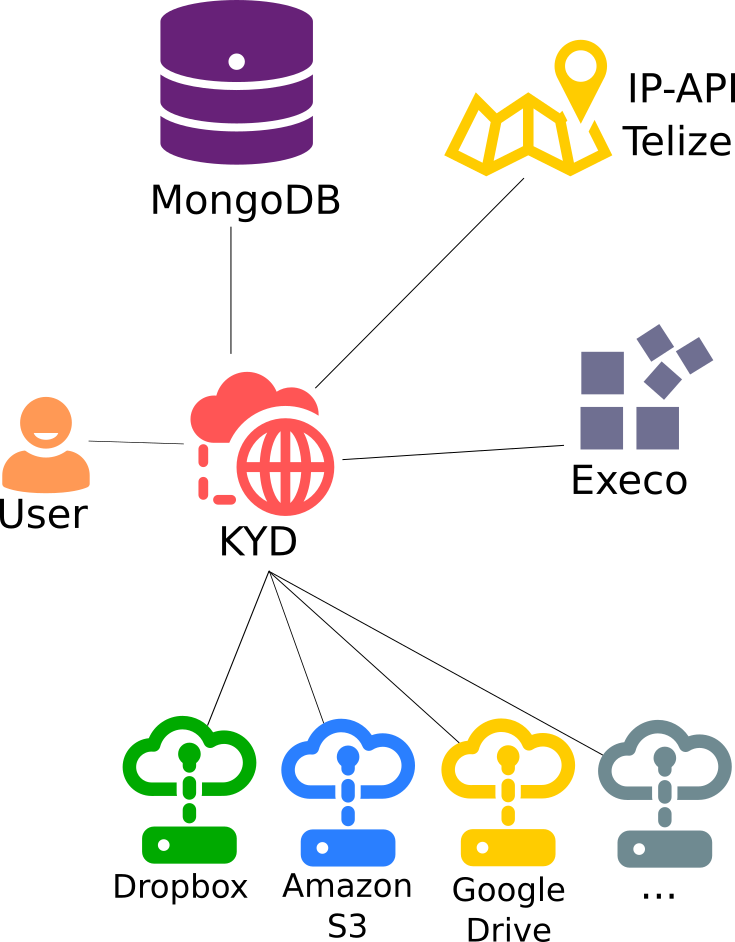
\includegraphics[scale=0.3]{architecture.png}
\caption{Graphe des downloads}
\label{fig:Graphe des downloads}
\end{figure}

\subsection{Améliorations}

À terme, plusieurs améliorations sont envisageables. Ajouter des
paramètres pour augmenter la précision des tests ferait partie de ces
améliorations\todo{YC : pourquoi, actuellement pas assez précis ? C'est une fausse question, mais justifier ce que vous écrivez}. Il serait par exemple possible de vérifier l'efficacité
des compte premium qui apportent peut être de meilleures
performances. Il faudrait également compléter la base de données pour
pouvoir répondre le plus souvent possible à l'utilisateur sans avoir à
lui faire effectuer des tests parfois coûteux en temps. Il serait
alors nécessaire d'effectuer des tests à plusieurs emplacements
géographiques dans le monde. Enfin, une interface Web plus conviviale
pourrait rapporter les résultats à l'utilisateur à la place de la
console. Cette amélioration se veut majoritairement esthétique mais
pourrait apporter un certain nombre de renseignements supplémentaires
à l'utilisateur\todo{YC : parlez d'ergonomie, de synthèse d'information}.

\section{Analyse des résultats}

Suite à de nombreux tests\todo{YC : décrivez calmement le protocol expérimental.
 Quels sont les paramètres communs examinés à toutes les expériences, quelles sont les caractéristiques qui ont changé, combien de tests ont été fait (parler d'intervalle si besoin).}

  , nous avons pu obtenir différentes courbes
traduisant les divers aspects de notre projet. Pour les figures 1 et
2, les tests ont été réalisés depuis le campus de la Doua à Lyon 1. Un
grand nombre de tests ont été effectués en "upload" et en "download"
avec une taille de fichier différente puis la moyenne\todo{YC : flou. Moyenne sur combien ?} de ces tests a
permis d'obtenir ces résultats.

\begin{figure}[h]
\centering
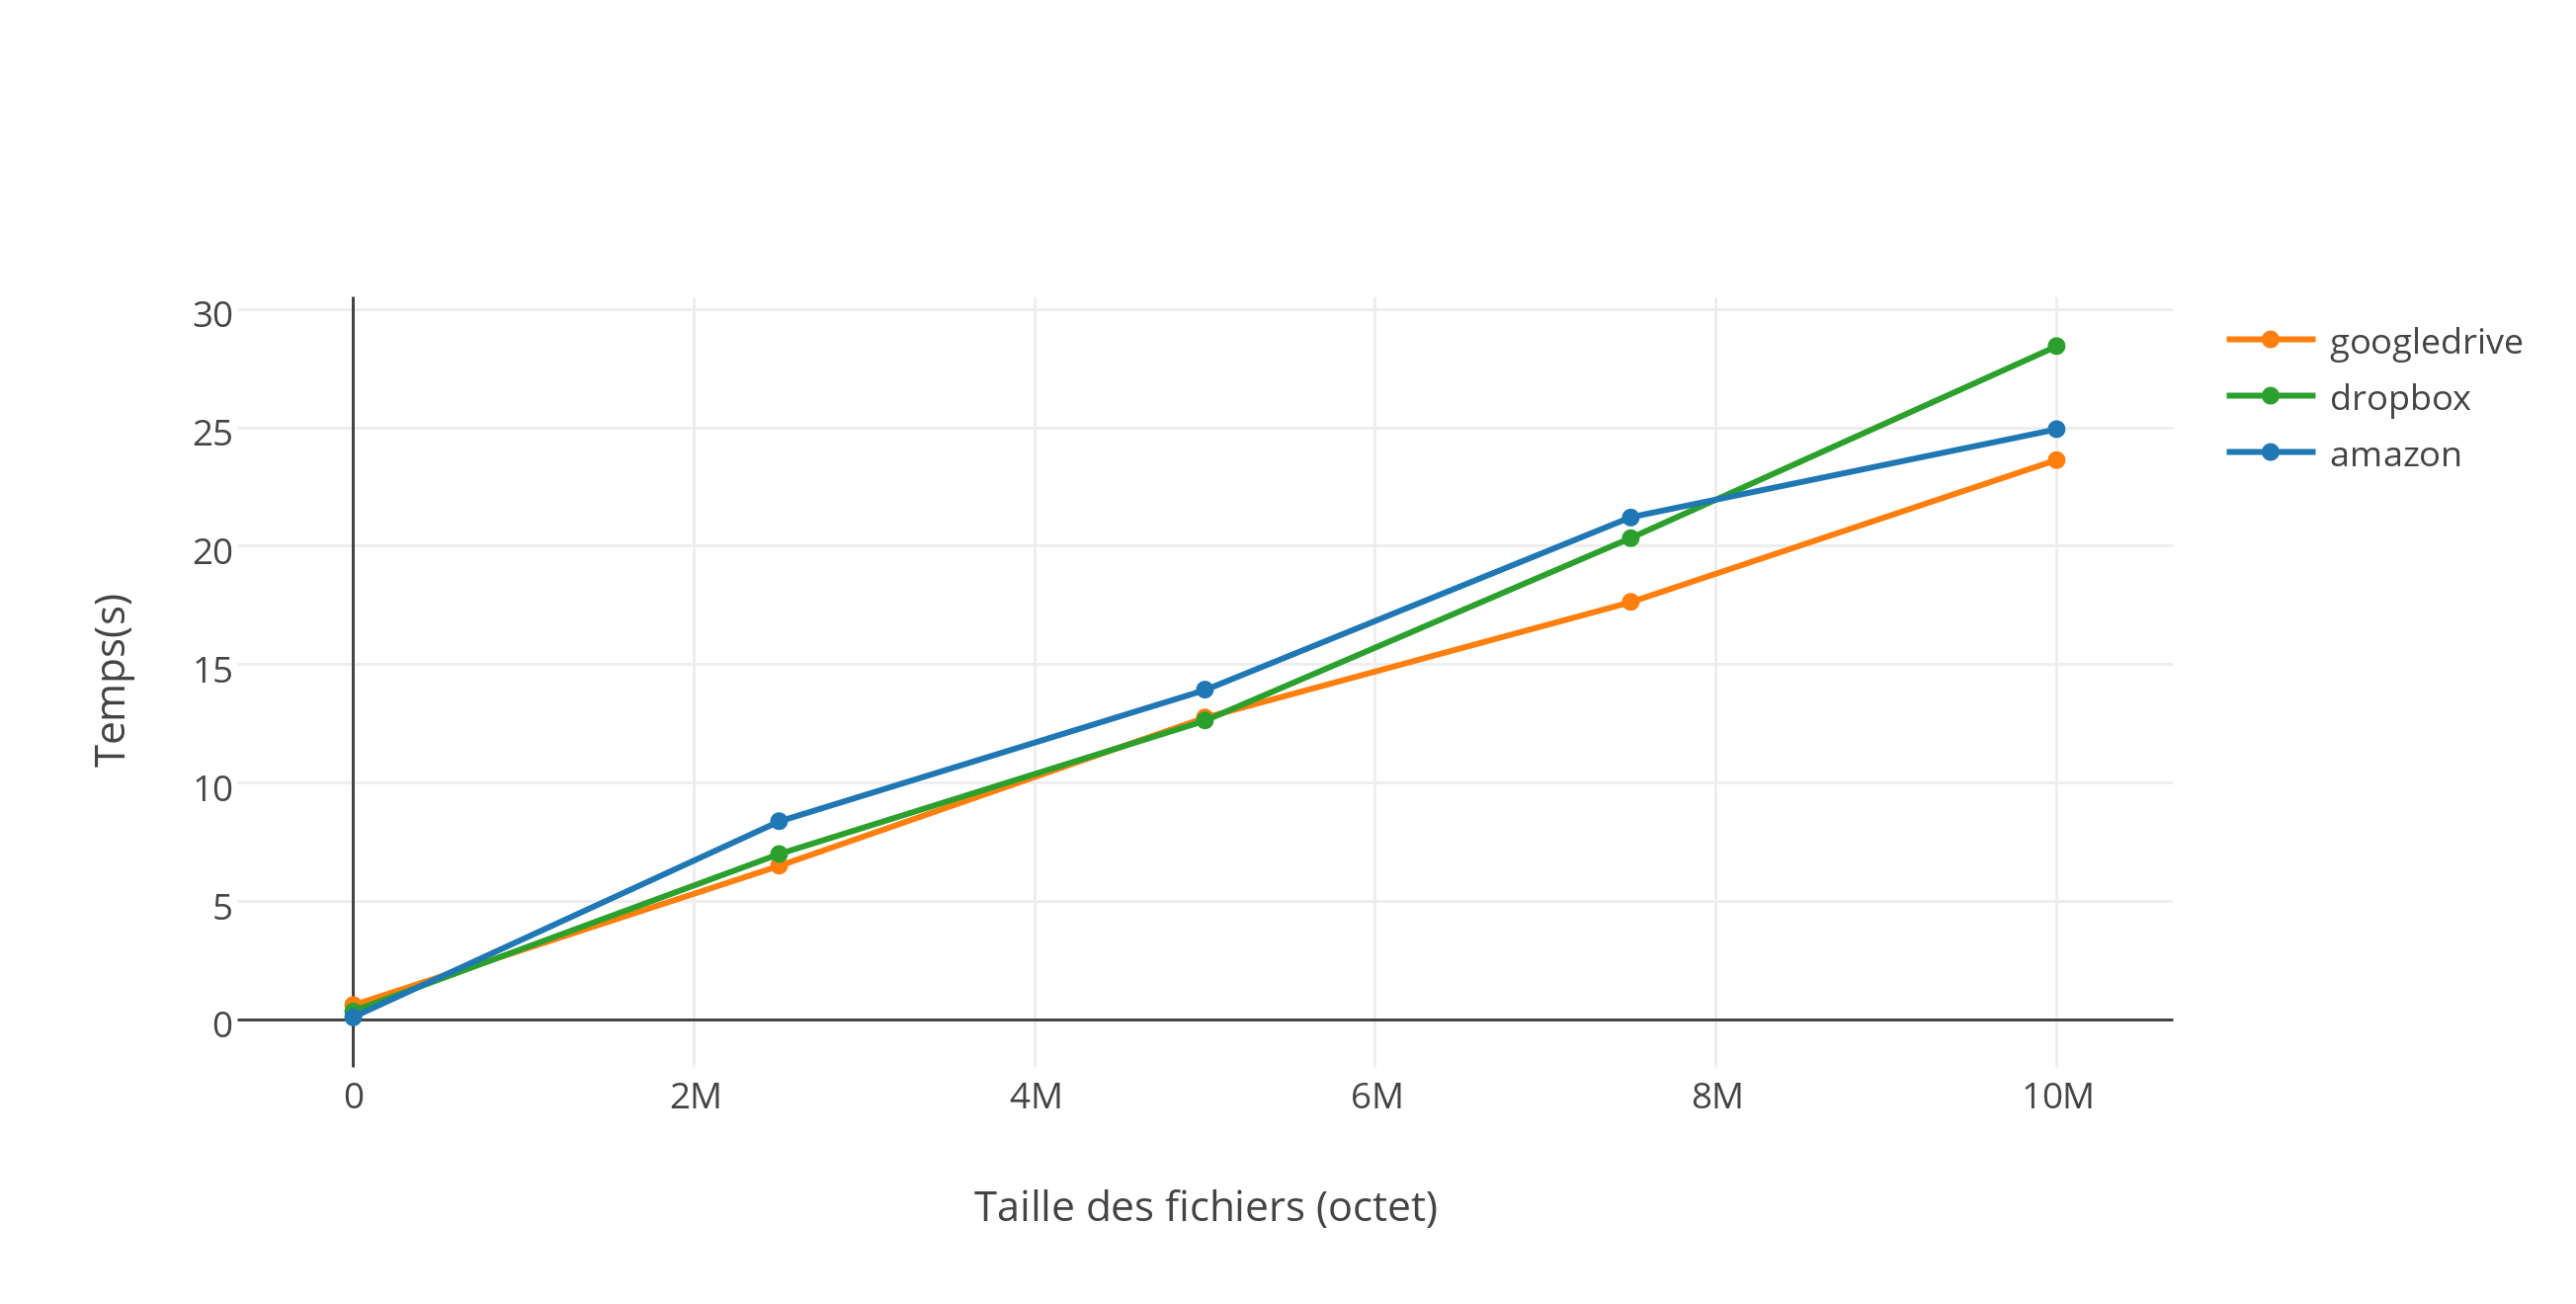
\includegraphics[scale=0.7]{graphe_des_downloads.png}
\caption{Graphe des downloads}
\end{figure}

\newpage

\begin{figure}[h]
\centering
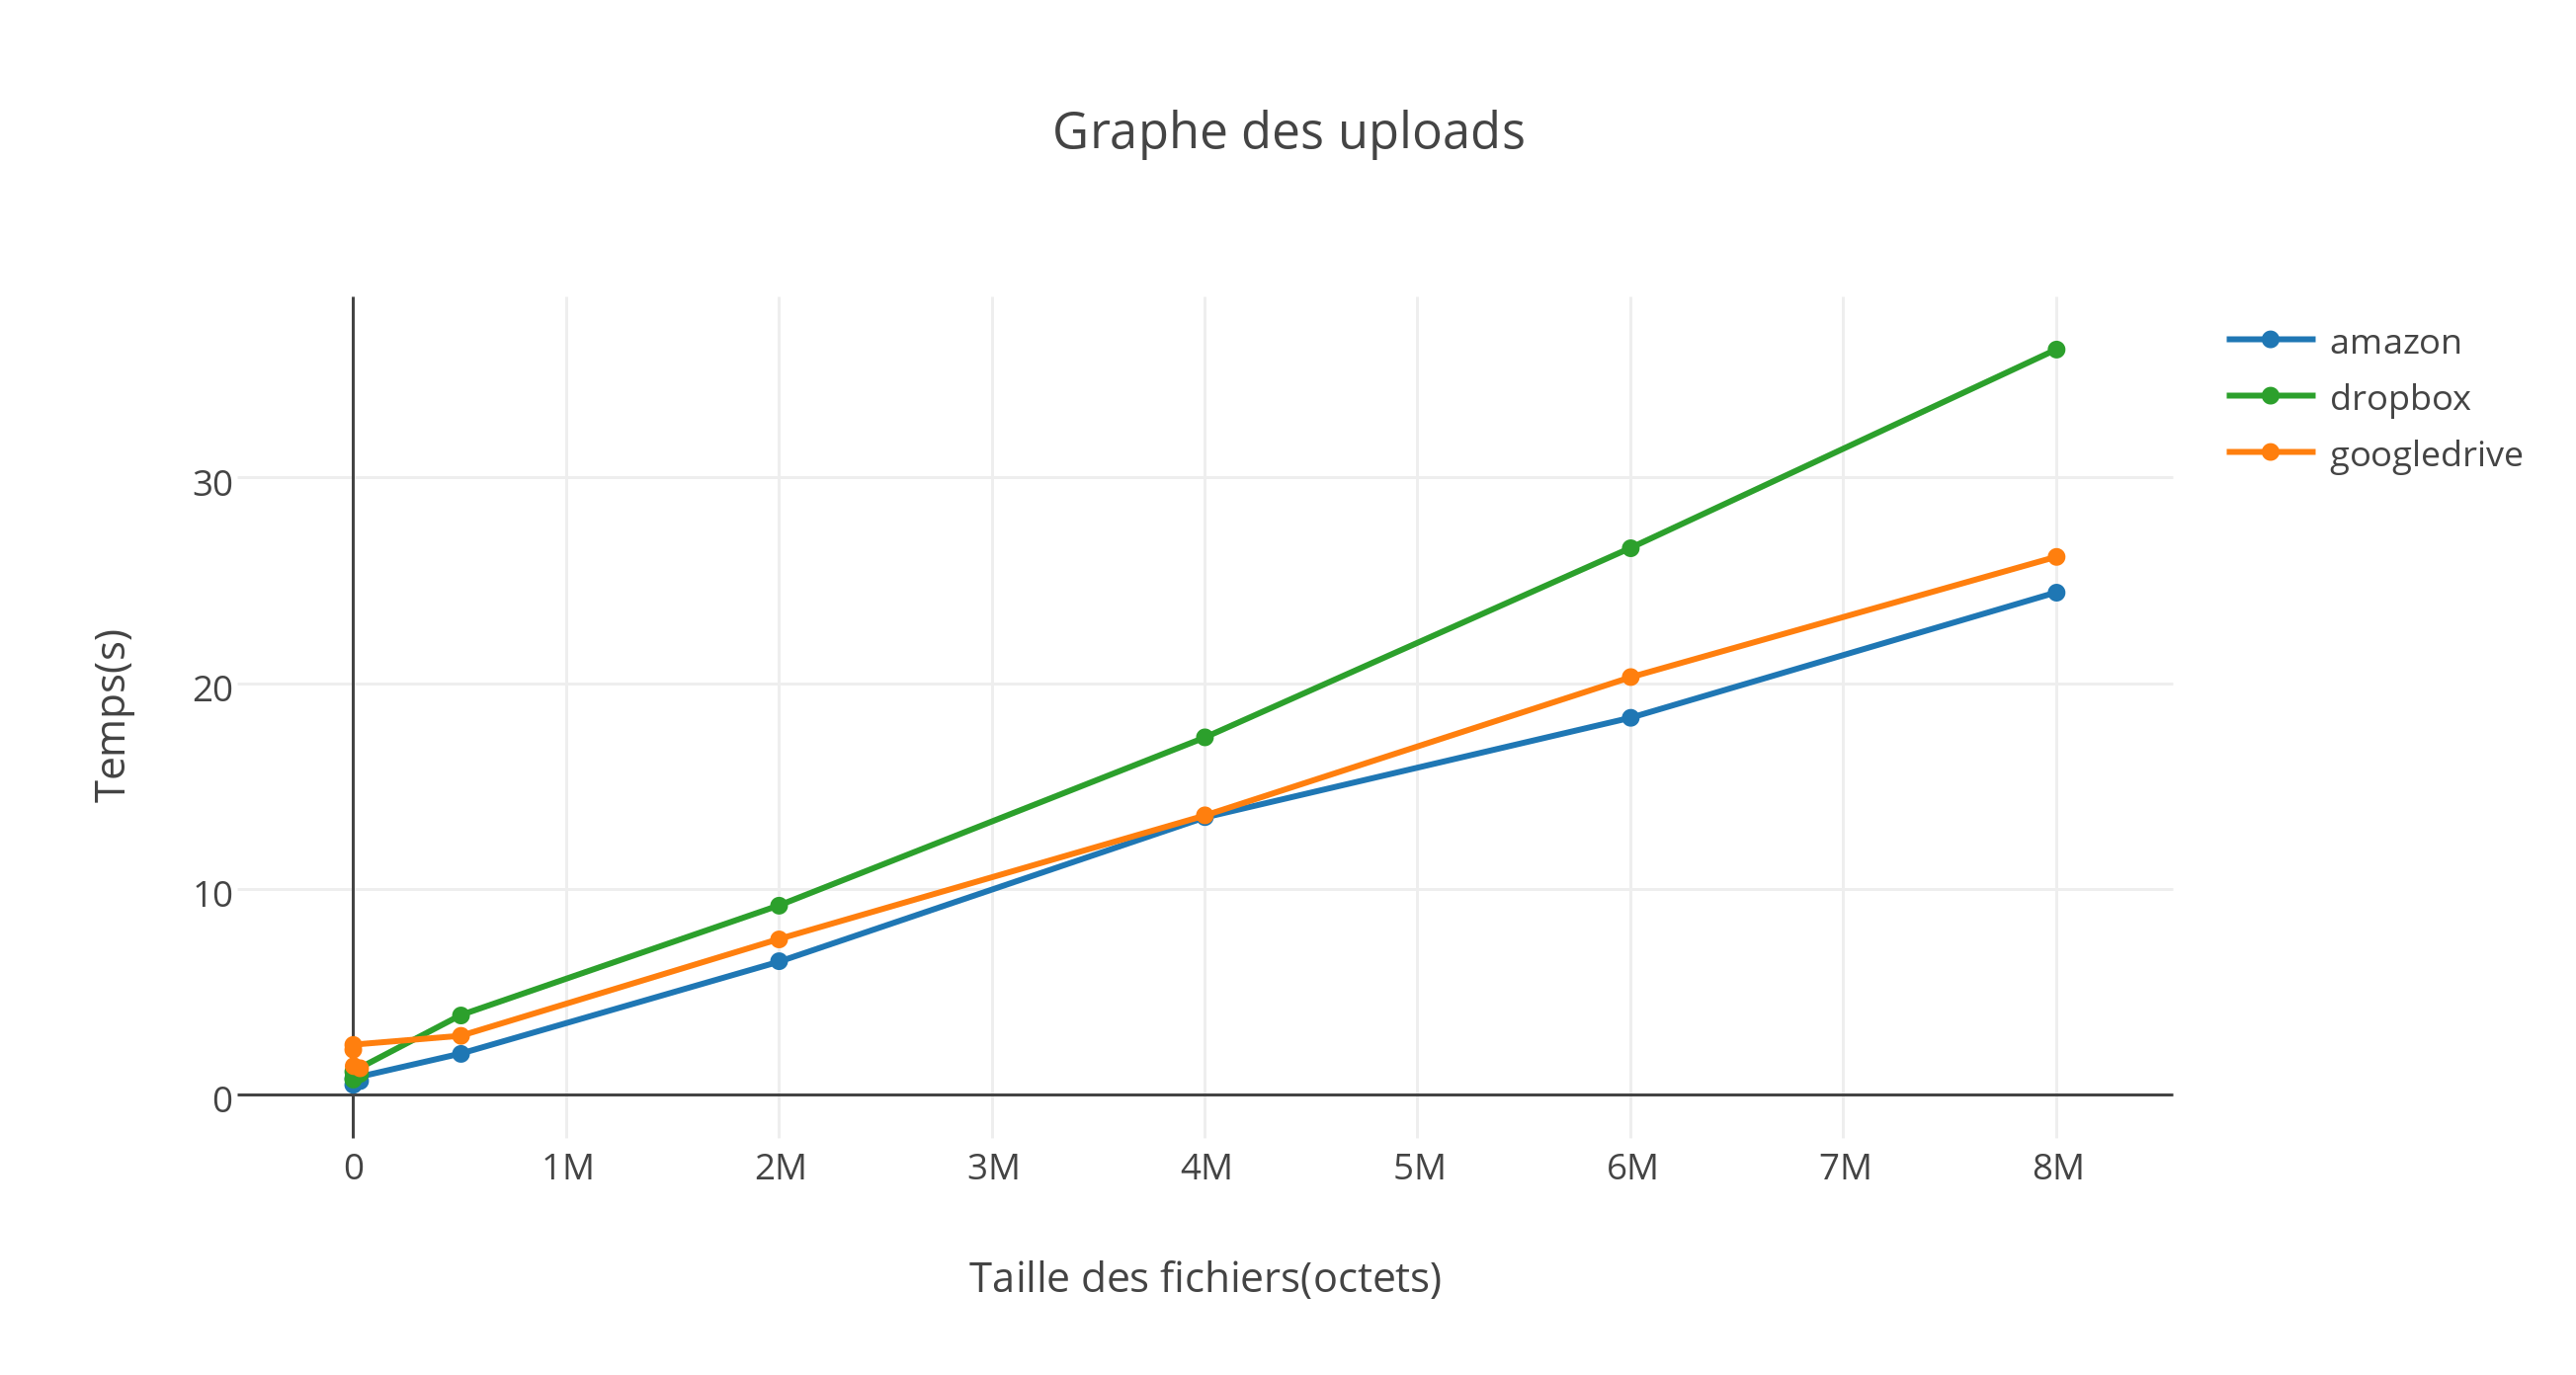
\includegraphics[scale=0.7]{graphe_des_uploads.png}
\caption{Graphe des uploads}
\end{figure}


Il est clairement visible\todo{YC : pê. Mais après que vous ayez présenté les courbes, et où le lecteur voit clairement ;) Et avec référence au(x) tableaux/graphes qui vont bien} que, dans cette situation, Dropbox est le
choix le moins pertinent sauf en ce qui concerne la connexion. Amazon
et Google Drive seront donc des choix beaucoup plus pertinents
puisqu'on peut observer une différence d'environ 20 points\todo{YC : des points ?} entre
Dropbox et ses deux concurrents en ce qui concerne les performances
(et cette différence ne cesse de croître avec l'augmentation de la
taille des fichiers).\\

Pour les deux figures suivantes, les tests ont été effectués depuis un
serveur virtuel situé à Londres. Ils ont été lancés toutes les heures
pendant vingt quatre heures un dimanche avec une taille de fichier de
10Mo à l'aide de la crontab du serveur.


\begin{figure}[h]
\centering
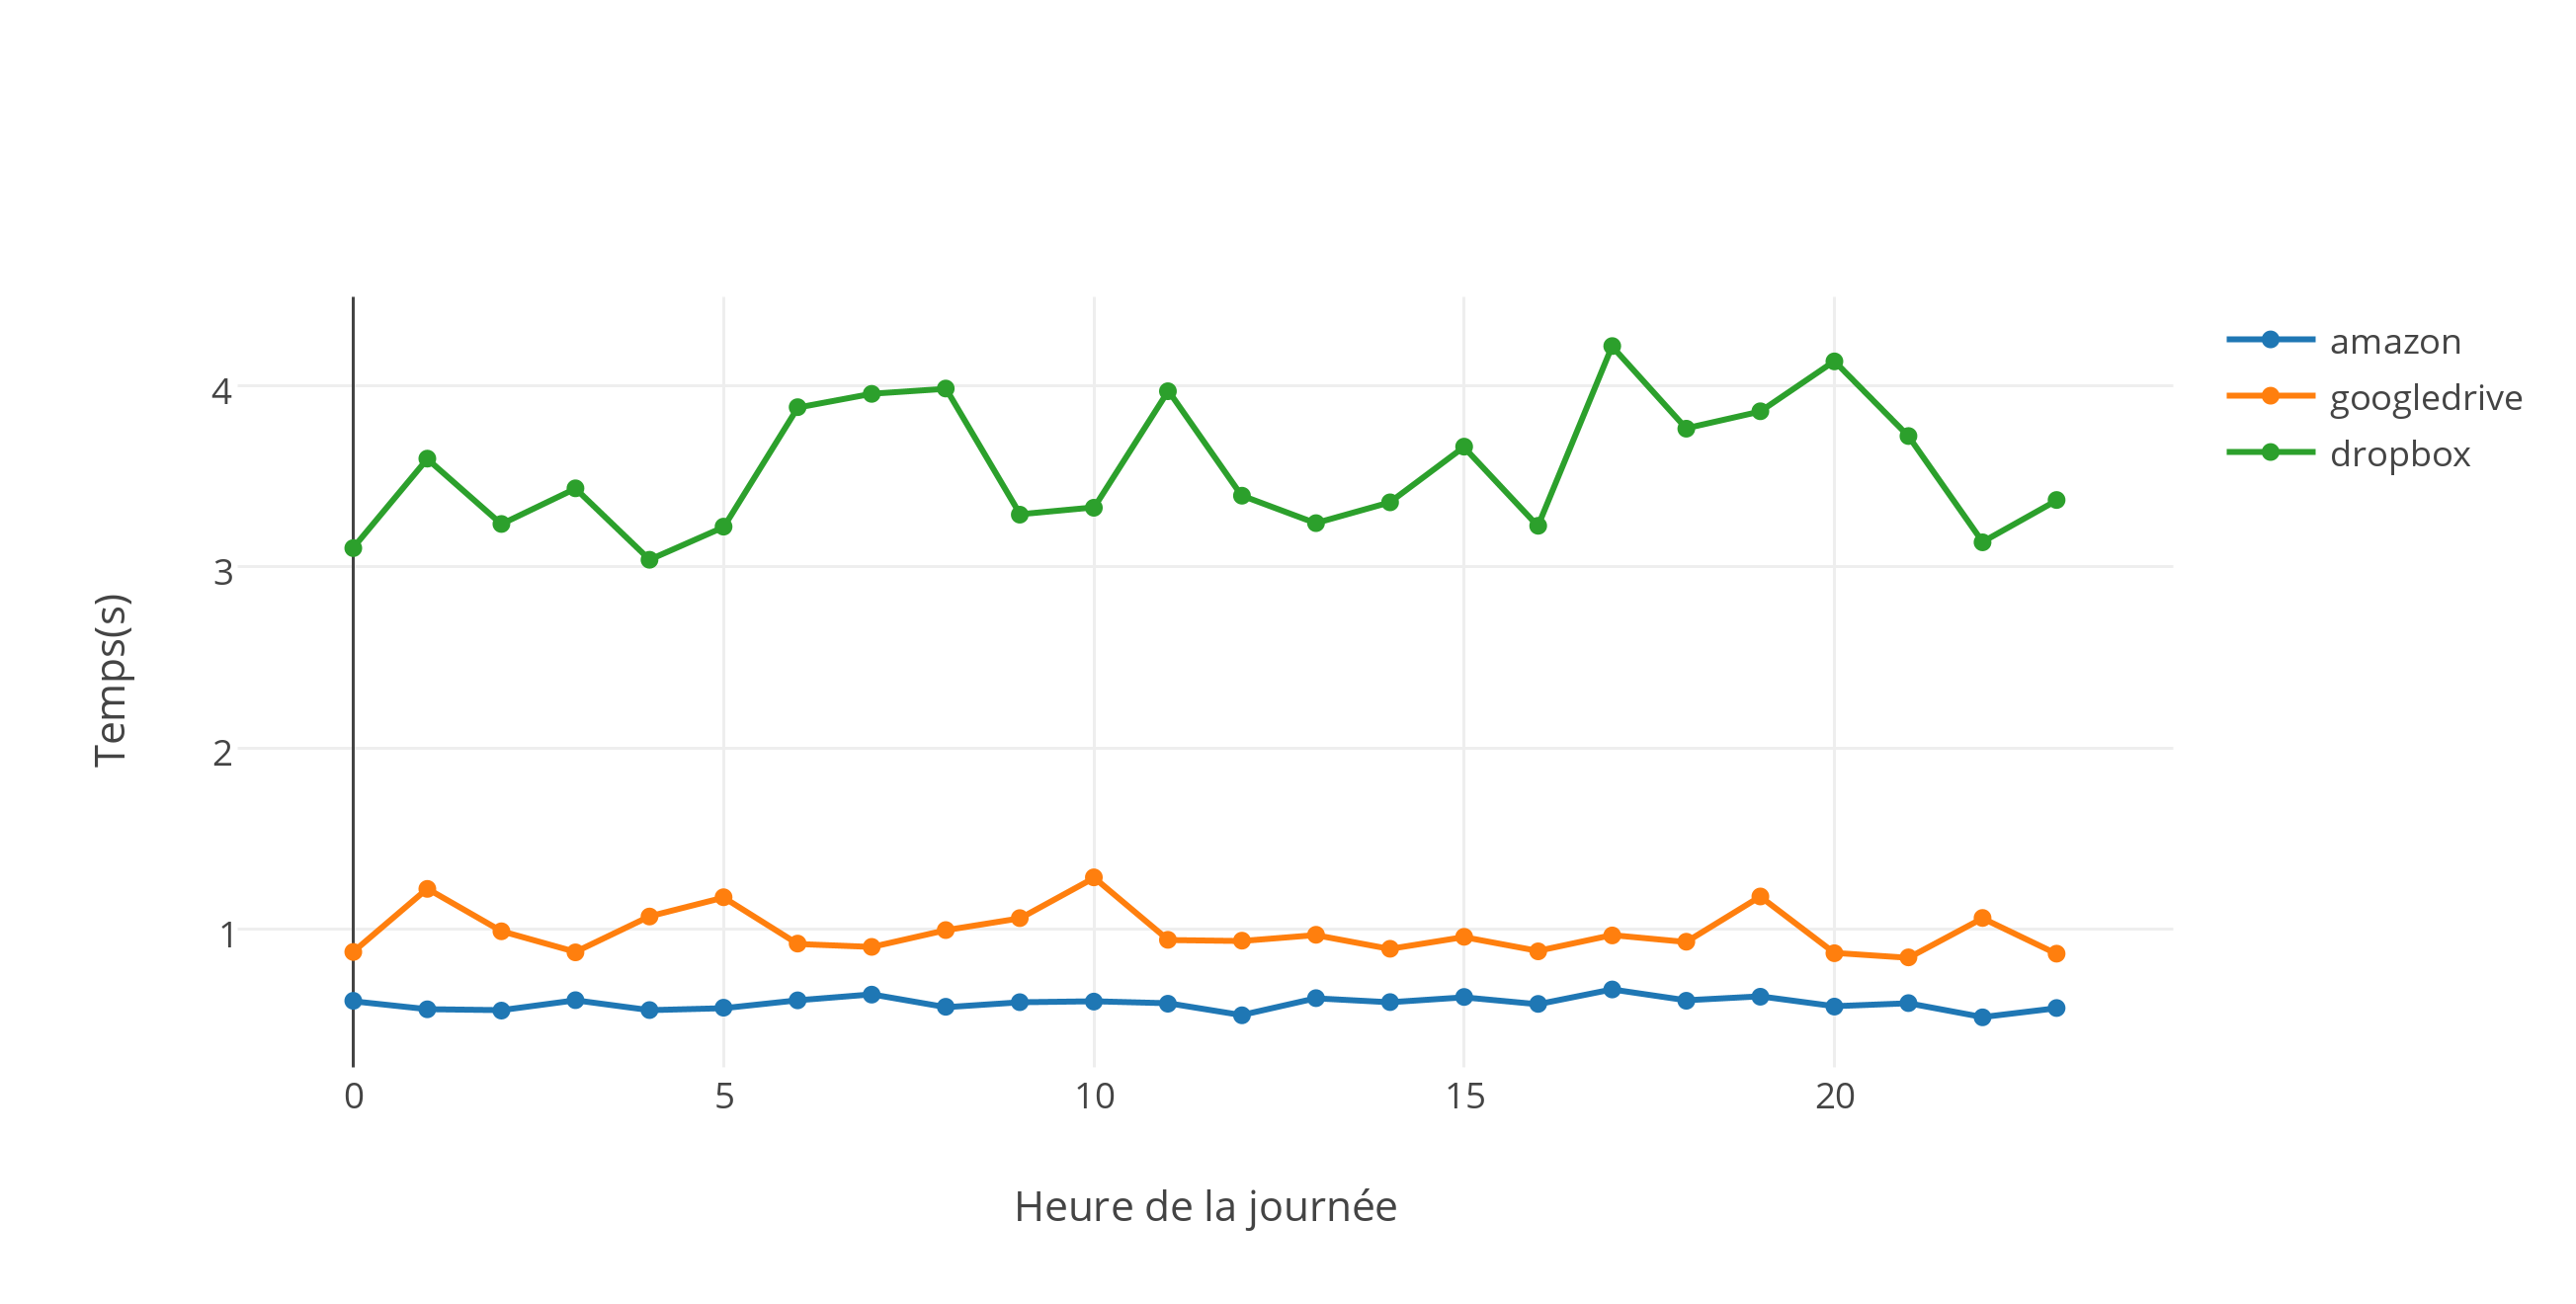
\includegraphics[scale=0.7]{graphe_du_15022015_pour_les_download_de_taille_10mo.png}
\caption{Graphe des downloads du 15 de taille 10Mo}
\end{figure}

\newpage

\begin{figure}[h]
\centering
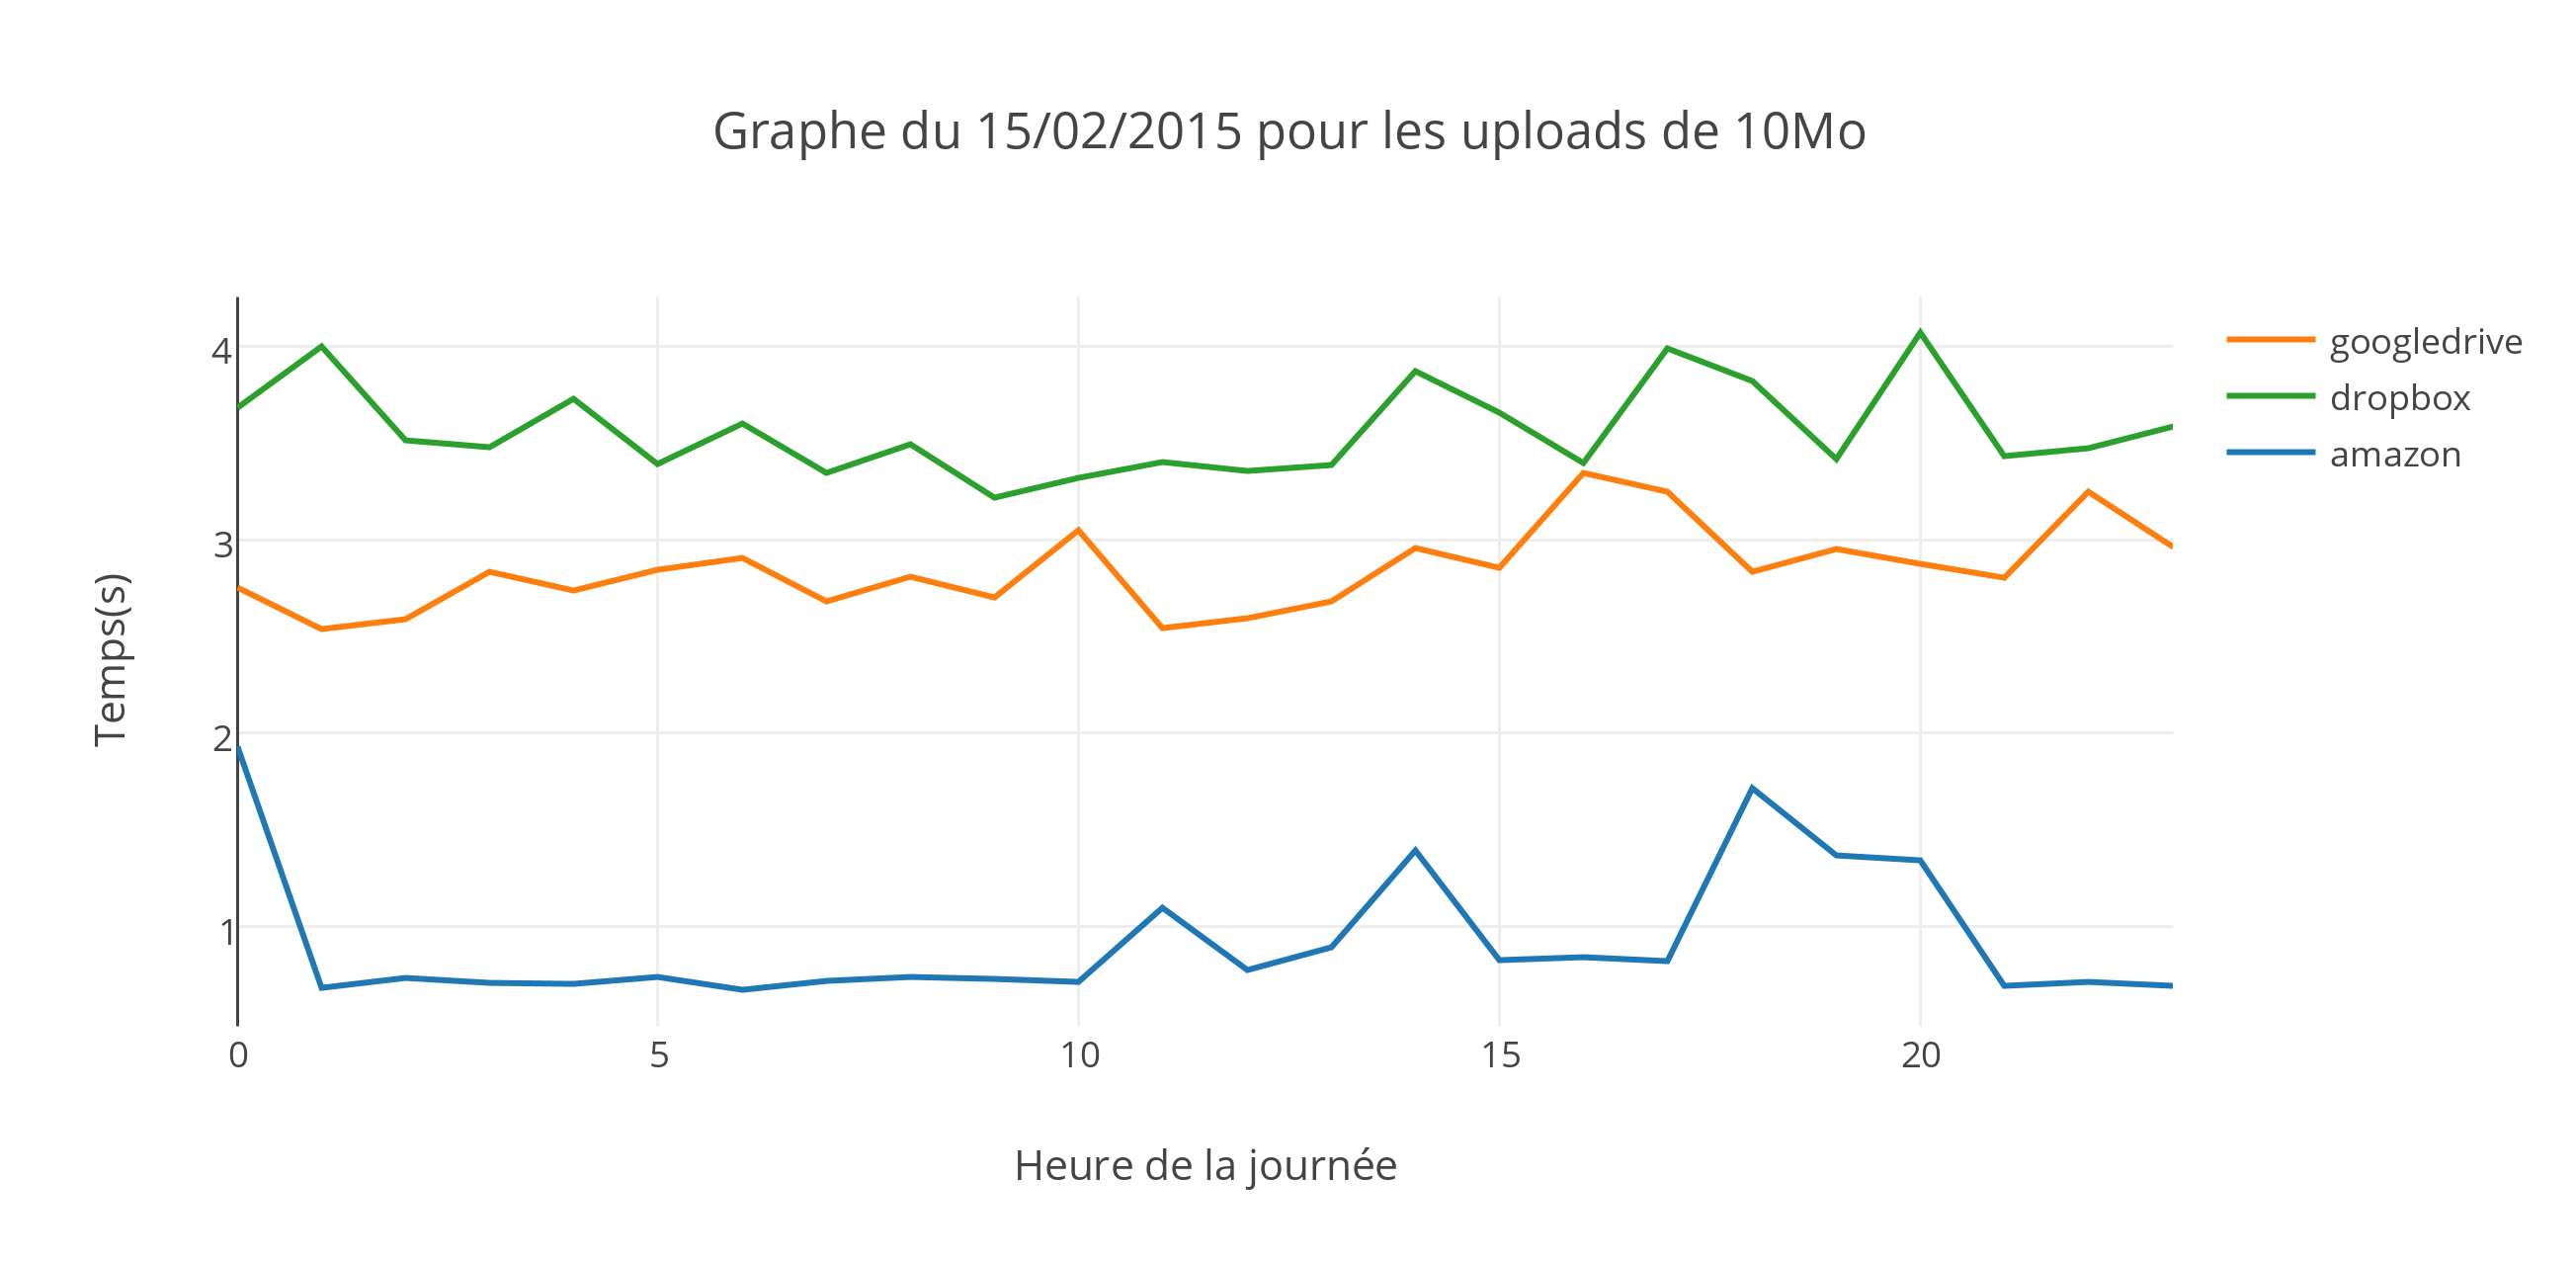
\includegraphics[scale=0.7]{graphe_du_15022015_pour_les_uploads_de_10mo.png}
\caption{Graphe des uploads du 15 de taille 10Mo}
\end{figure}


En "upload", on observe qu'Amazon suit un schéma connu qui comporte
des pics de latence à 11h, 14h puis entre 18h et 20h. On suppose que
cette situation est due au grand nombre de connexions simultanées
durant une plage horaire plus bondée que les autres. Les performances
de Dropbox sont, cette fois encore, très nettement inférieures à
celles de ses concurrents.
\todo{YC : du bon commentaire. J'en veux d'autres ! ;D}


\section{Conclusion}

\section{Annexes}

Ce que vous avez vu, ce sur quoi vous vous êtes formés, des choses que
vous avez apprises (travail d'initiation à la recherche, l'évaluation
devrait aussi comporter un paragraphe en annexe sur vos impressions,
votre retour d'expérience).

\end{document}
